\SetTitle{2}{Reversible Computations}{No energy lost or gained}{reverse}

\begin{frame}{Overview}
\begin{itemize}
    \item Quantum computations involve gates that are \emph{unitary} and therefore are invertible.
    \item Quantum computations are delicate and noise must be kept to a minimum.  Interactions with the environment will cause the quantum system to collapse (\href{https://en.wikipedia.org/wiki/Quantum_decoherence}{decoherence}).
    \item We study a mechanical computer first where it is clear that a nonreversible computation gains or loses energy.
    \item We can build reversible circuits for classical and quantum computations.
    
\end{itemize}
\end{frame}

\begin{frame}{The \href{https://en.wikipedia.org/wiki/Billiard-ball_computer}{billiard ball computer}}{When a single ball enters at a time}
\TwoColumns{%
Consider the mechanical \emph{and} gate shown here.
\begin{itemize}
    \item<1-> A ball entering from the top
    \only<2->{will emerge from the ``1-out'' hole.}
    \item<3-> A ball entering from the left
    \only<4->{will emerge from the ``0-out'' hole.}
    
\end{itemize}
}{%

\begin{TIKZP}
\node at (0,0)
    {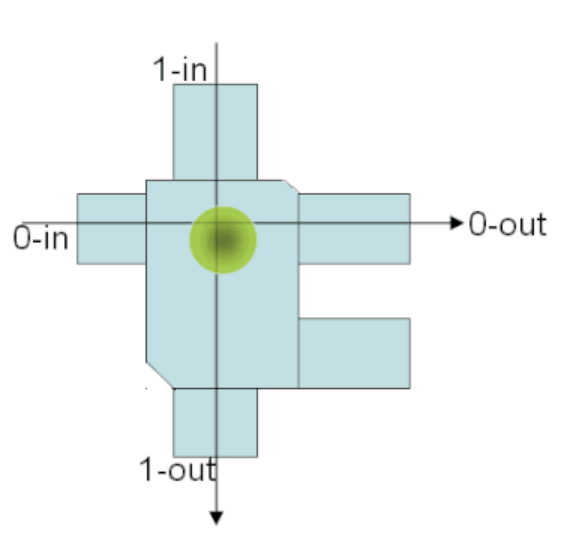
\includegraphics[width=0.7\textwidth]{2/single.png}};
\visible<1>{\fill[color=SpringGreen] (-.59,2.2) circle(0.25);}
\visible<2>{\fill[color=SpringGreen] (-.59,-2.1) circle(0.25);}
\visible<3>{\fill[color=SpringGreen] (-2.7,0.3) circle(0.25);}
\visible<4>{\fill[color=SpringGreen] (2.5,0.3) circle(0.25);}
\end{TIKZP}

}
\only<5->{
\MedSkip{}No energy is put in or taken out of the system.  The ball has its own energy, maintained throughout its motion through the box.}
    
\end{frame}
\begin{frame}{The billiard ball computer}{When two balls enter simultaneously}
\TwoUnequalColumns{0.6\textwidth}{0.4\textwidth}{%
Here, two balls enter, one from the top, and one from the left
\begin{itemize}
    \item<1-> A ball entering from the top and a ball entering from the left at the same time
    \only<2->{will \alert<2>{collide here}.}
    \item<3-> They bounce internally at the same time.
    \item<4-> One ball emerges from the ``AND-output'' chute and the other emerges from the ``1-out'' chute.
    
\end{itemize}
}{%
\Vskip{-3.2em}\Hskip{-0em}
\begin{TIKZP}
\node at (0,0)
    {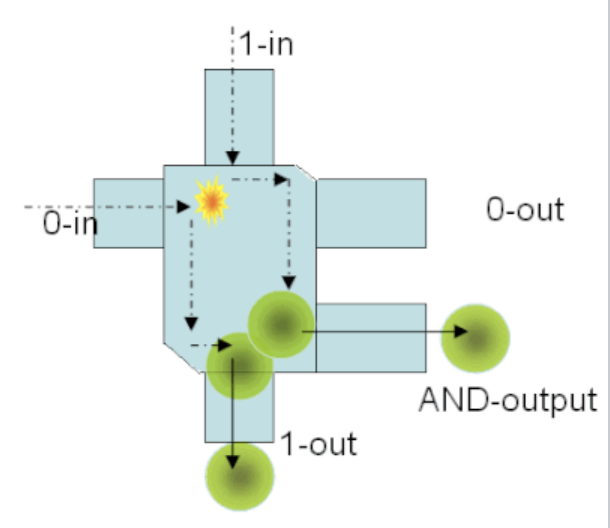
\includegraphics[width=0.7\textwidth]{2/double.png}};
\visible<1>{\fill[color=SpringGreen] (-.45,1.8) circle(0.25);}
\visible<2>{\fill[color=red] (-.6,0.4) circle(0.25);}
\visible<1>{\fill[color=SpringGreen] (-2.2,0.3) circle(0.25);}
\end{TIKZP}

}
\only<5->{
\SmallSkip{}Again, the energy of the box remains the same throughout.\Remark{It would take energy to \emph{stop} the ball from exiting the ``1-out'' chute.}}

    
\end{frame}